\documentclass[biblatex,aspectratio=169,11pt]{mybeamer}

\usetikzlibrary{backgrounds,calc,decorations.pathreplacing,fit,matrix,patterns,positioning,shapes,shapes.multipart,tikzmark}
\makeatletter
\let\@@magyar@captionfix\relax
\makeatother

%Add page footer
\setbeamertemplate{footline}[text line]{%
  \parbox{\linewidth}{\vspace*{-8pt}\hfill CS6290 Privacy-enhancing Technologies\hfill\insertpagenumber}}
\setbeamertemplate{navigation symbols}{}

\title{A Preliminary Study on Stateless Blockchain}
\author{Yang Ji}
\date{April 15, 2019}

\addbibresource{ref.bib}

\begin{document}

\maketitle%
\PrintTOC%

\section{Introduction}

\begin{frame}{Background}
  \begin{itemize}
    \item In cryptocurrency, peer-to-peer payment transactions are asynchronously broadcasted and recorded in an ordered ledger.
    \item Consensus protocol requires nodes to validate new transactions. 
    \item e.g. To send 6 ETC from Alice to Bob requires that Alice has at least 6 ETC.
    \item Simply querying the history from adjacent nodes is infeasible and insecure due to the large size of blocks.
    \item For that reason, most cryptocurrency nodes need to locally maintain the \alert{ledger state}, which means downloading all past transactions/accounts.
  \end{itemize}
\end{frame}

\begin{frame}{Background}
  \begin{itemize}
    \item In Bitcoin, Zcash and Komodo, \alert{validation state} is a set of immutable coins called \alert{UTXO} (unspent transaction output)
  \end{itemize}
  \vspace{-1em}
  \begin{figure}
    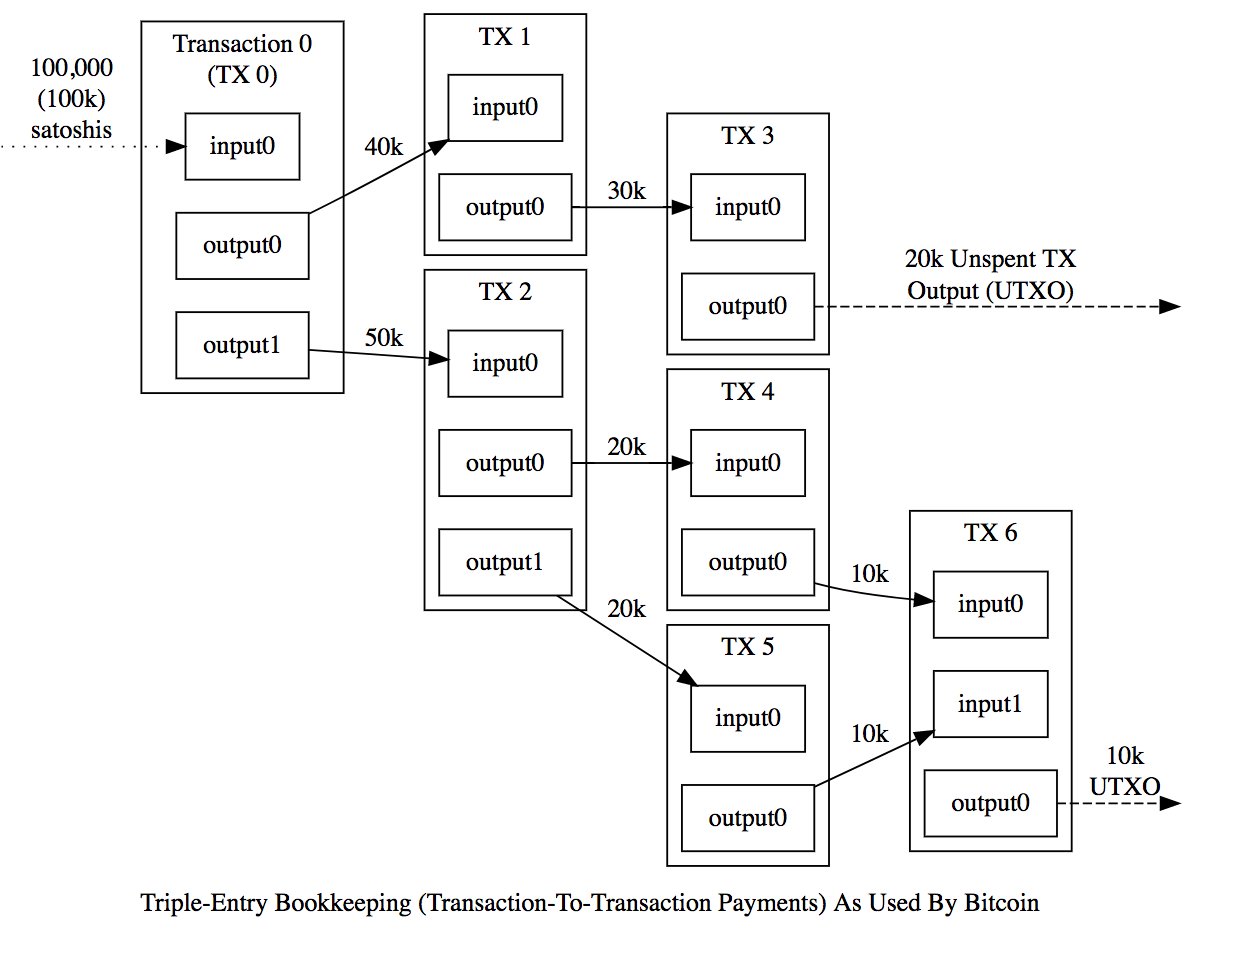
\includegraphics[width=0.45\linewidth]{figs/utxo.png}
    \caption{UTXO Model}
  \end{figure}
\end{frame}


\begin{frame}{Background}
  \begin{itemize}
    \item In Ethereum, Nxt and Bitshares organize \alert{validation state} as a set of mutable (and potential long-living) \alert{accounts}.
  \end{itemize}
  \vspace{-1em}
  \begin{figure}
    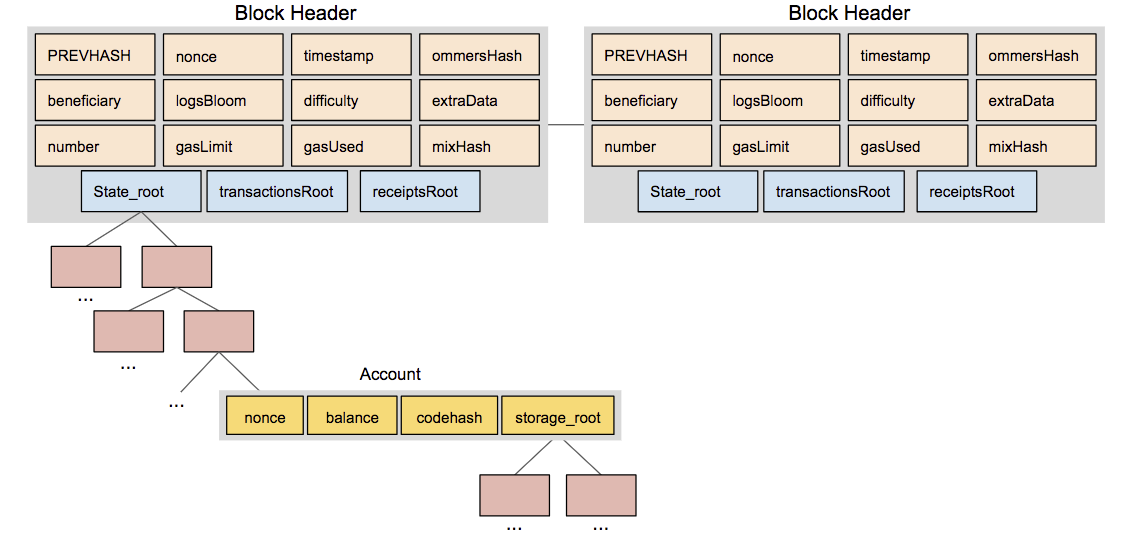
\includegraphics[width=0.7\linewidth]{figs/account.png}
    \caption{Account-based Model}
  \end{figure}
\end{frame}

\begin{frame}{background}
  \begin{itemize}
    \item Other cryptocurrencies
  \end{itemize}
  \vspace{-1em}
  \begin{figure}
    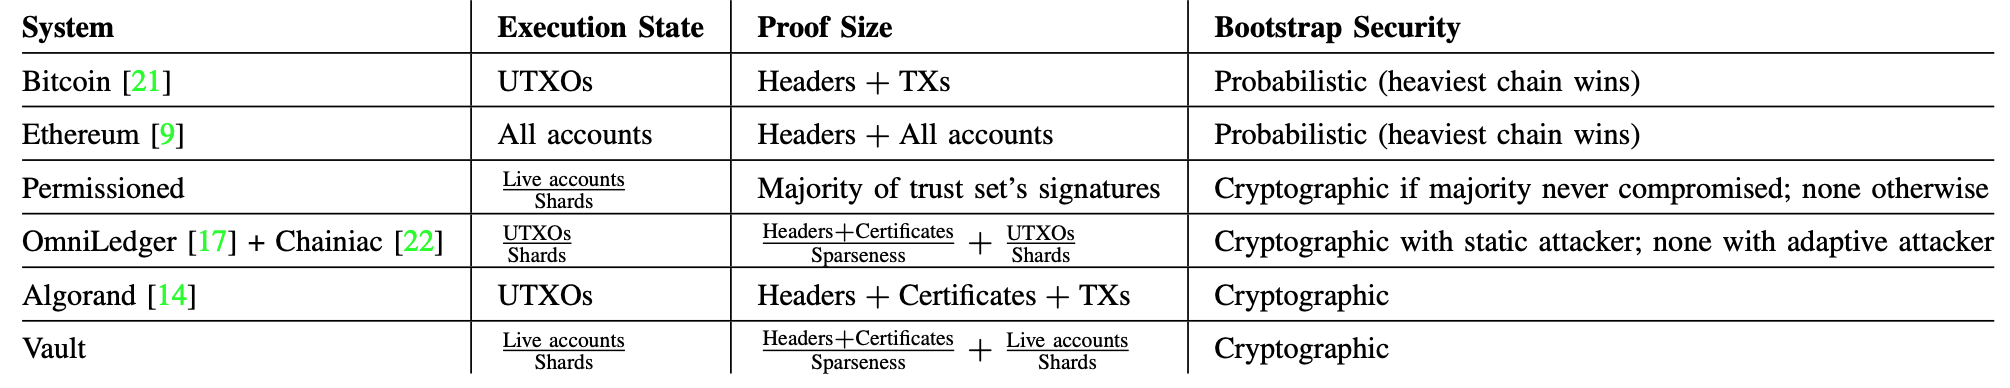
\includegraphics[width=0.9\linewidth]{figs/summary.png}
    \caption{Comparison of different cryptocurrency models }
  \end{figure}
\end{frame}

\begin{frame}{Motivation}
  \begin{itemize}
    \item Maintaining ledger state is cumbersome from the perspectives of \alert{storage} and \alert{bootstrapping}
    \begin{itemize}
       \item Large size (Bitcoin is around 150 GB and Ethereum has exceeded 400 GB)
       \item Data storage size is linear with block number and could grow substantially in the coming years
       \item Slow disk I/O operations (LevelDB or RocksDB)
       \item DoS attack (adversarially-crafted transactions that need massive of disk accesses)
       \item Increase the possibility of centralization in blockchains.
    \end{itemize}
    \item It thus appears that we need to remove the \alert{ledger state} and allow miners to validate pending transactions without storing all past blocks. 
  \end{itemize}
\end{frame}

\begin{frame}{Stateless Blockchain}
   \begin{itemize}
    \item This design concept of \alert{Stateless Blockchain} is referred to Peter Todd's blog post~\cite{Tod}. 
    \item Nodes might participate in transaction validation without storing the entire state of the ledger.
    \item Several people including Peter Todd and Mike Hearn also talked about stateless clients for Bitcoin in 2013. Back to then, they call it \alert{Storageless}.
    \item Many optimized schemes are put forward in the forum, such as Merkle Mountain tree~\cite{MMR} and asynchronous accumulator~\cite{reyzin2016efficient} for dual accumulator.
  \end{itemize}
\end{frame}

\begin{frame}{Difficulty}
  \begin{itemize}
    \item Currently the maximum size of the UTXO/Account set is unbounded as there is no consensus rule that limits growth.
    \item State set growth is driven by a number of factors, including the following fact.
     \begin{itemize}
       \item For \alert{Bitcoin}, there are massive of merge inputs, lost coins and dust outputs.
       \item For \alert{Ethereum}, smart contract inadvertently created many \alert{zero-balance accounts}~(account for around 38\%).
     \end{itemize}
    \item Based on these, a na\"ive way is to prune and clean `useless' dust coins/accounts.
    \item However, there is little incentive to carry it out for many reasons:
     \begin{itemize}
       \item Dust coins can't be economically spent and have other use cases.
       \item We can't delete zero accounts because nodes need to keep track of the sequence number ("nonce")~\cite{wood2014ethereum}.
     \end{itemize}
    \item There is little space for optimizing index structures and storage mode.
  \end{itemize}
\end{frame}

\section{Analysis of Existing works}

\begin{frame}{Categories}
  \begin{itemize}
    \item Method 1: \alert{Storage rent}
     \begin{itemize}
       \item Miner could outsource her local database to a third party.
     \end{itemize}
    \item Method 2: \alert{Sharding}
     \begin{itemize}
       \item Partition the whole blockchain/storage into many shards.
     \end{itemize}
    \item Method 3: \alert{Commitment to the ledger state}
      \begin{itemize}
        \item Transaction would include membership proofs for all its input.
        \item A node would only need to store the current state and verify transactions by checking membership proofs against accumulator state.
      \end{itemize}
  \end{itemize}
\end{frame}

\section{Stateless Blockchain}

\metroset{subsectionpage=simple}
\subsection{\fullcite{leung2019vault}}

\begin{frame}{Vault Techniques}
  \begin{itemize}
    \item \textbf{Vault:} Reducing the cost of storage and bootstrapping without weakening security guarantees.
  \end{itemize}
  \vspace{-2em}
  \begin{table}[]
    \begin{tabular}{|l|l|l|}
    \hline
    Approach                                                                                 & Challenge                                                               & Vault’s Solution                                                        \\ \hline
    \begin{tabular}[c]{@{}l@{}}Reduce state\\ transmitted:\\ Garbage collection\end{tabular} & \begin{tabular}[c]{@{}l@{}}Transaction replay\\ attacks\end{tabular}    & \begin{tabular}[c]{@{}l@{}}Force transactions\\ to expire\end{tabular}  \\ \hline
    \begin{tabular}[c]{@{}l@{}}Reduce state\\ transmitted:\\ Shard state\end{tabular}        & \begin{tabular}[c]{@{}l@{}}Small shards lose\\ security\end{tabular}    & \begin{tabular}[c]{@{}l@{}}Adaptive Merkle\\ Tree sharding\end{tabular} \\ \hline
    \begin{tabular}[c]{@{}l@{}}Reduce size of\\ state proof:\\ Compress history\end{tabular} & \begin{tabular}[c]{@{}l@{}}Attacker tampers\\ with history\end{tabular} & \begin{tabular}[c]{@{}l@{}}Succinct\\ certificates\end{tabular}         \\ \hline
    \end{tabular}
  \end{table}
\end{frame}

\begin{frame}{Vault: Forcing Transactions to Expire}
  \begin{itemize}
    \item All transactions contain the fields \alert{$t_{issuance}$} and \alert{$t_{expiry}$}.
    \item We define $0 \leq t_{expiry} - t_{issuance} \leq t_{max}$
    \item The choice of $T_{max}$ affects two considerations.
     \begin{itemize}
       \item The block number of transactions to detect double spend.
       \item Expiration mechanism requires the issuer to reissue expired transactions.
     \end{itemize}
    \item Support off-chain payment channels e.g. Lightning Network.
  \end{itemize}
\end{frame}

\begin{frame}{Vault: Sharding Balance Storage}
  \vspace{-2em}
  \begin{figure}
    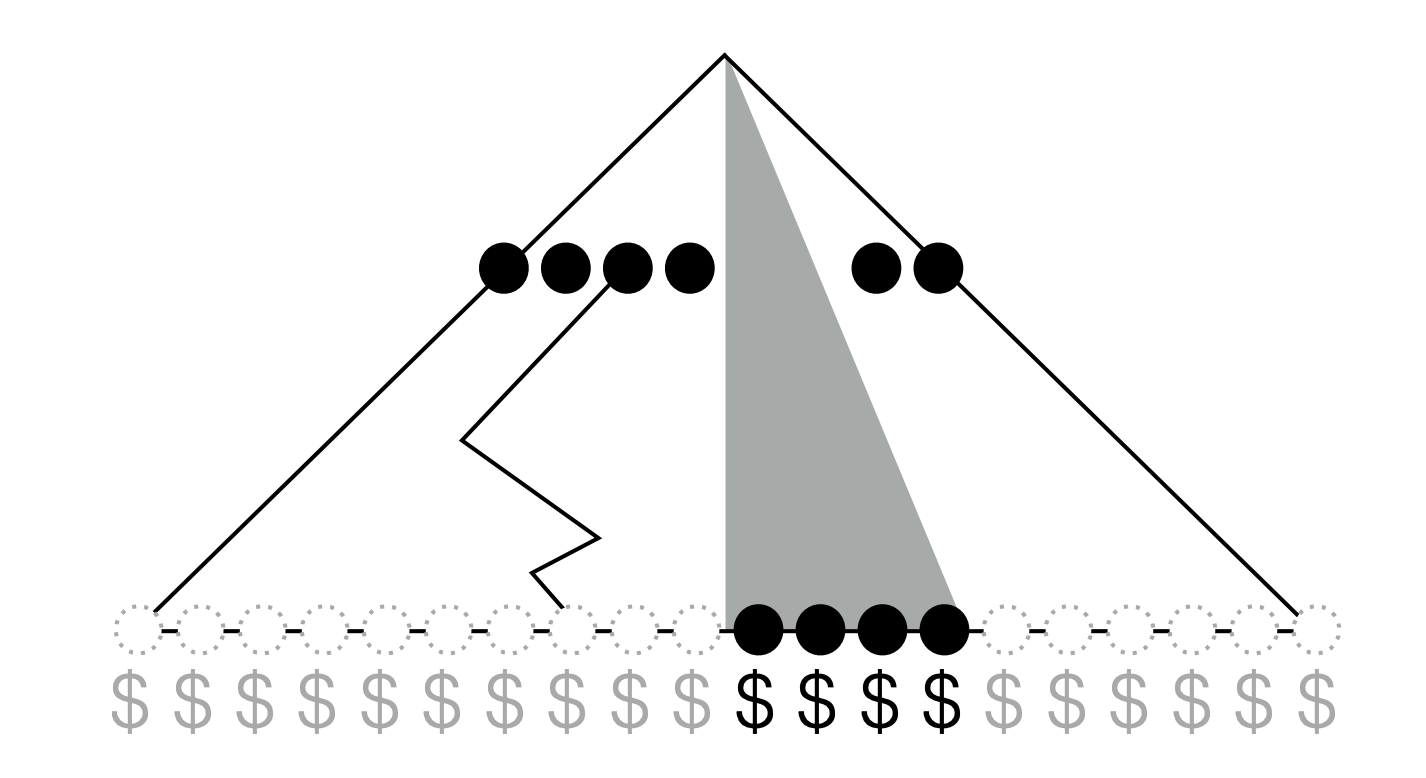
\includegraphics[width=0.5\linewidth]{figs/vault-sharding.png}
  \end{figure}
  \vspace{-2em}
  \begin{itemize}
    \item \textbf{Shard Witness:} Transactions include Merkle witness for source and destination accounts.
    \item \textbf{Updating Witness:} The witness could be updated without requiring the issuer to resign the entire transaction.
    \item \textbf{Adaptive Sharding: } Truncating witness.
  \end{itemize}
\end{frame}

\begin{frame}{Vault: Compressing History}
  \begin{itemize}
    \item Skipping Blocks
    \begin{figure}
      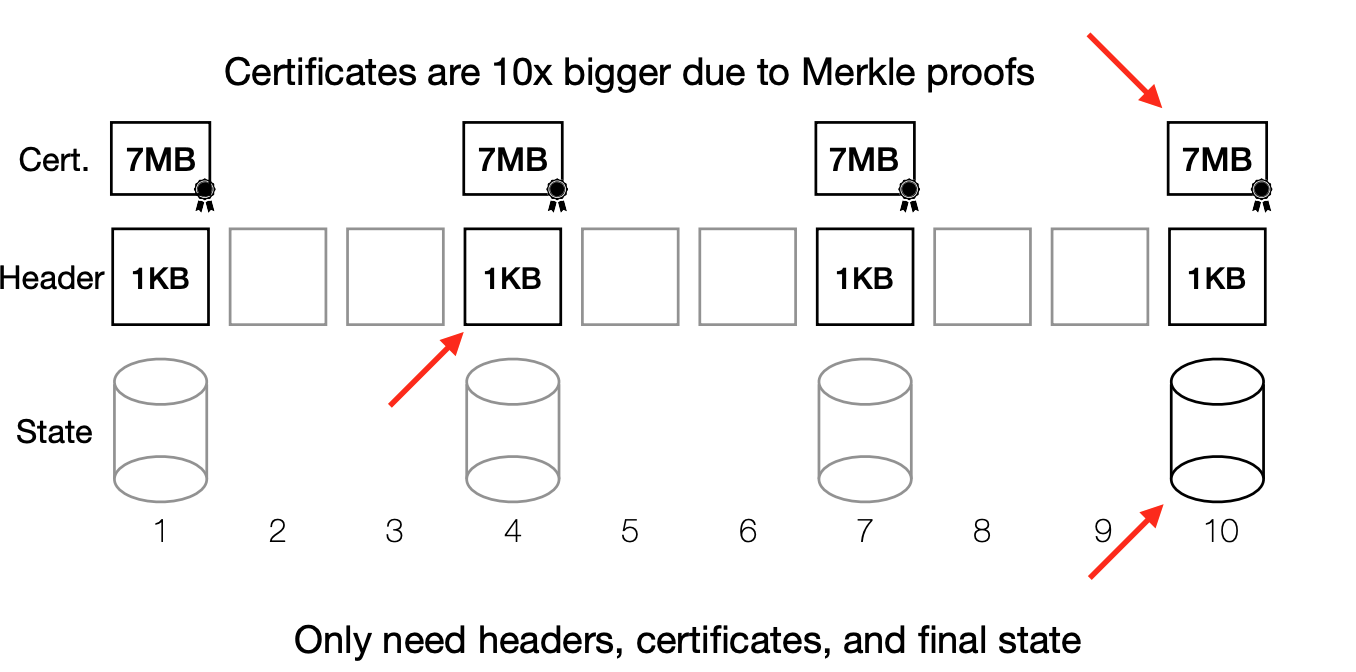
\includegraphics[width=0.5\linewidth]{figs/skip-block.png}
      \caption{An illustration for skipping blocks}
    \end{figure}
    \item Shrinking Certificates
  \end{itemize}
\end{frame}

\subsection{\fullcite{chepurnoy2018edrax}}

\begin{frame}{EDRAX Architecture}
  \begin{figure}
    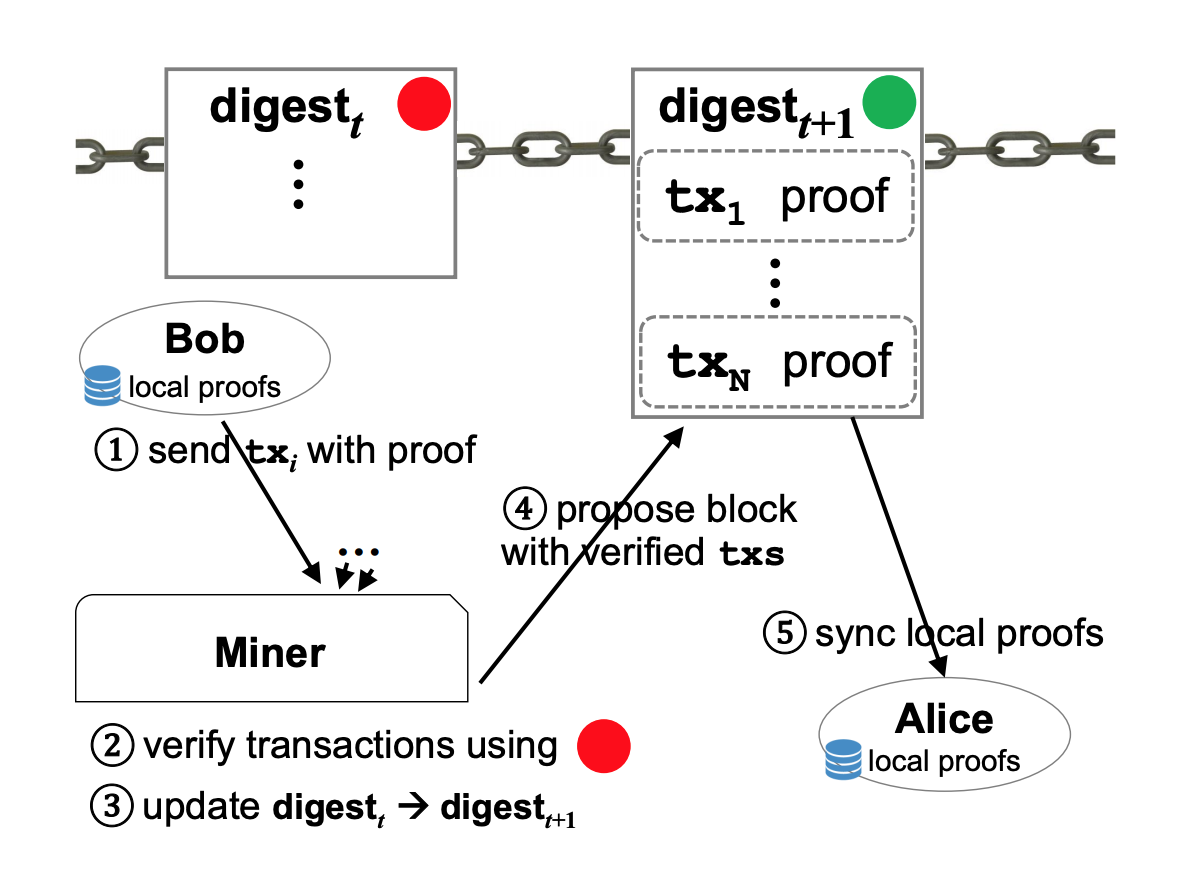
\includegraphics[width=0.6\linewidth]{figs/Edrax-arch.png}
    \caption{An illustration for skipping blocks}
  \end{figure}
\end{frame}

\begin{frame}{General Idea}
  \begin{itemize}
    \item Use vector commitment to represent the mapping of $pk \leftrightarrow balance$
    \item Store the vector commitment in the block as digest
    \item During \texttt{SPEND}
      \begin{itemize}
        \item Client submits a proof that $\mathcal{V}[sender] = v$
        \item Miner checks that $\delta \leq v$
        \item Miner updates digest by $\mathcal{V}[sender] = v - \delta, \mathcal{V}[reciver] = \mathcal{V}[reciver] + \delta$
        \item Clients update their proofs accordingly
      \end{itemize}
  \end{itemize}
\end{frame}

\nocite{*}
\PrintRef%
\PrintQA%

\end{document}
